\section{Actividad}

\subsection*{Identificación de devanados:}

Es necesario realizar algunas medidas preliminares. Estas comprenden la identificación de los bornes y verificación de su marcación. En este laboratorio se tomarán estas respectivas medidas de las máquinas de corriente continua que se encuentran en el laboratorio de Máquinas 1: Shunt y Compound.
\begin{figure}[ht!]
    \centering
    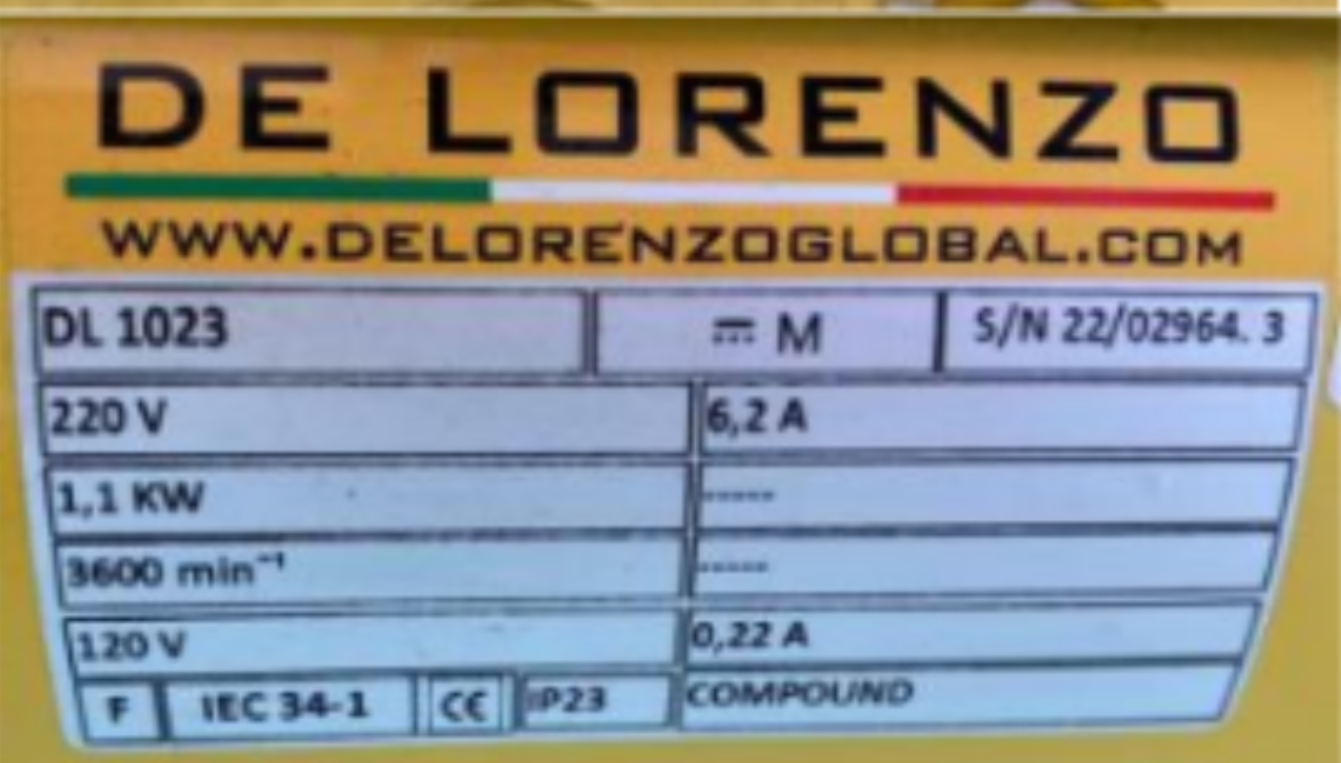
\includegraphics[width=0.48\textwidth]{fot/Prac_6_compound.png}
    \caption{Motor compound del laboratorio.}
    \label{fig:compound}
\end{figure}
\begin{figure}[ht!]
    \centering
    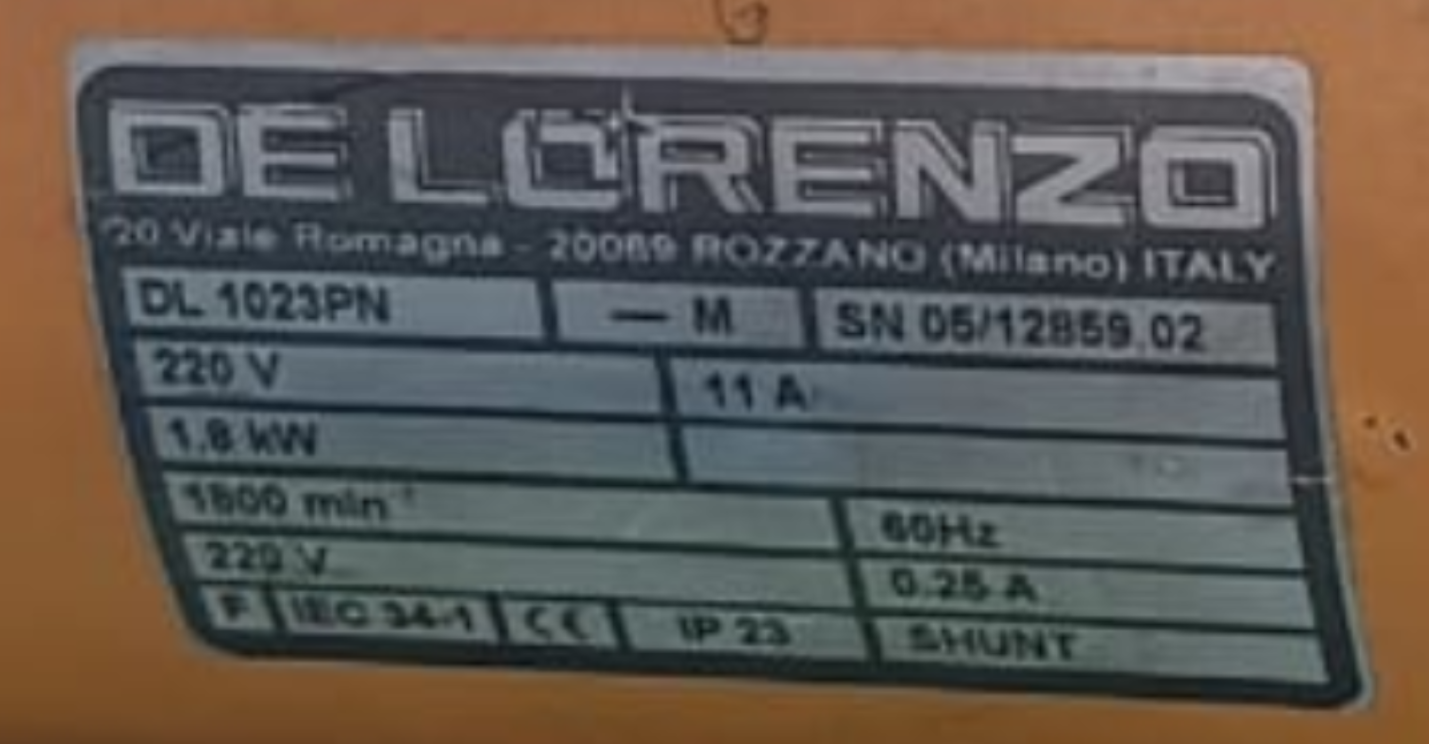
\includegraphics[width=0.48\textwidth]{fot/Prac_6_shunt.png}
    \caption{Motor shunt del laboratorio.}
    \label{fig:shunt}
\end{figure}
Para la identificación de los bornes usaremos un multímetro con el que podremos verificar la continuidad de cada uno de los bornes, con eso sabremos cuáles son los bornes a los que tendremos que medirles su valor resistivo. Para identificarlos, tendremos que tener los siguientes puntos en cuenta:

\begin{itemize}
    \item El devanado de campo shunt tiene el mayor valor resistivo de todos los devanados.
    
    \item El devanado de armadura se hace girar el eje, porque si en los bornes medidos se induce tensión, así sea un poco, ese sería el devanado de armadura.
    
    \item Para este devanado teníamos también acceso a las escobillas, con este también se podría identificar directamente.
    
    \item Para identificar el devanado de campo serie se tiene que aplicar unos pulsos en el devanado shunt y donde se encuentre la mayor tensión en los devanados no identificados, ese sería el devanado de campo serie.
\end{itemize}

Este procedimiento se realizará para cada una de las máquinas que tenemos en el laboratorio: Shunt, Compuesta. Como la identificación de los bornes no requiere de procedimientos complejos, los instrumentos y equipos que usaremos en el laboratorio serán un multímetro.

\subsection*{Resistencia en los devanados (shunt)}

\begin{tabular}{|c|c|c|}
\hline
DEVANADO & VALOR ($\Omega$) & BORNES \\
\hline
ARMADURA & 3.5 & A1-B2 \\
SHUNT & 8.77 & E1-E2 \\
\hline
\end{tabular}

\subsection*{Resistencia de aislamiento (shunt)}

\begin{tabular}{|c|c|c|}
\hline
VALOR (G$\Omega$) & BORNES \\
\hline
7.45 & A1 - TIERRA \\
926 & E2 - TIERRA \\
5.49 & B2 – E2 \\
\hline
\end{tabular}

\subsection*{Resistencia en los devanados (Compound)}

\begin{tabular}{|c|c|c|}
\hline
DEVANADO & VALOR ($\Omega$) & BORNES \\
\hline
ARMADURA & 2.7 & A1 – B2 \\
SERIE & 0.5 & D1 – D2 \\
SHUNT & 0.570 (k) & E1 – E2 \\
\hline
\end{tabular}

\subsection*{Resistencia de aislamiento (Compound)}

\begin{tabular}{|c|c|c|}
\hline
VALOR (G$\Omega$) & BORNES \\
\hline
18.8 & A1 - TIERRA \\
20.9 & D1 - TIERRA \\
4.75 & E1 – TIERRA \\
4.93 & A1 – D1 \\
1.94 & A1 – E1 \\
4.47 & D1 – E1 \\
\hline
\end{tabular}

Para la siguiente parte del laboratorio usaremos el esquema que se nos indicó en la guía de la práctica, el cual es tomar el voltaje y corriente del devanado de armadura (Ra, Va, Ia) con eso generar una tabla y esa misma tabla se extrapolará para poder encontrar el valor aproximado de la caída de tensión en las escobillas.

El esquema que se piensa usar es el siguiente (figura \ref{fig:modelol}).
\begin{figure}[ht!]
    \centering
    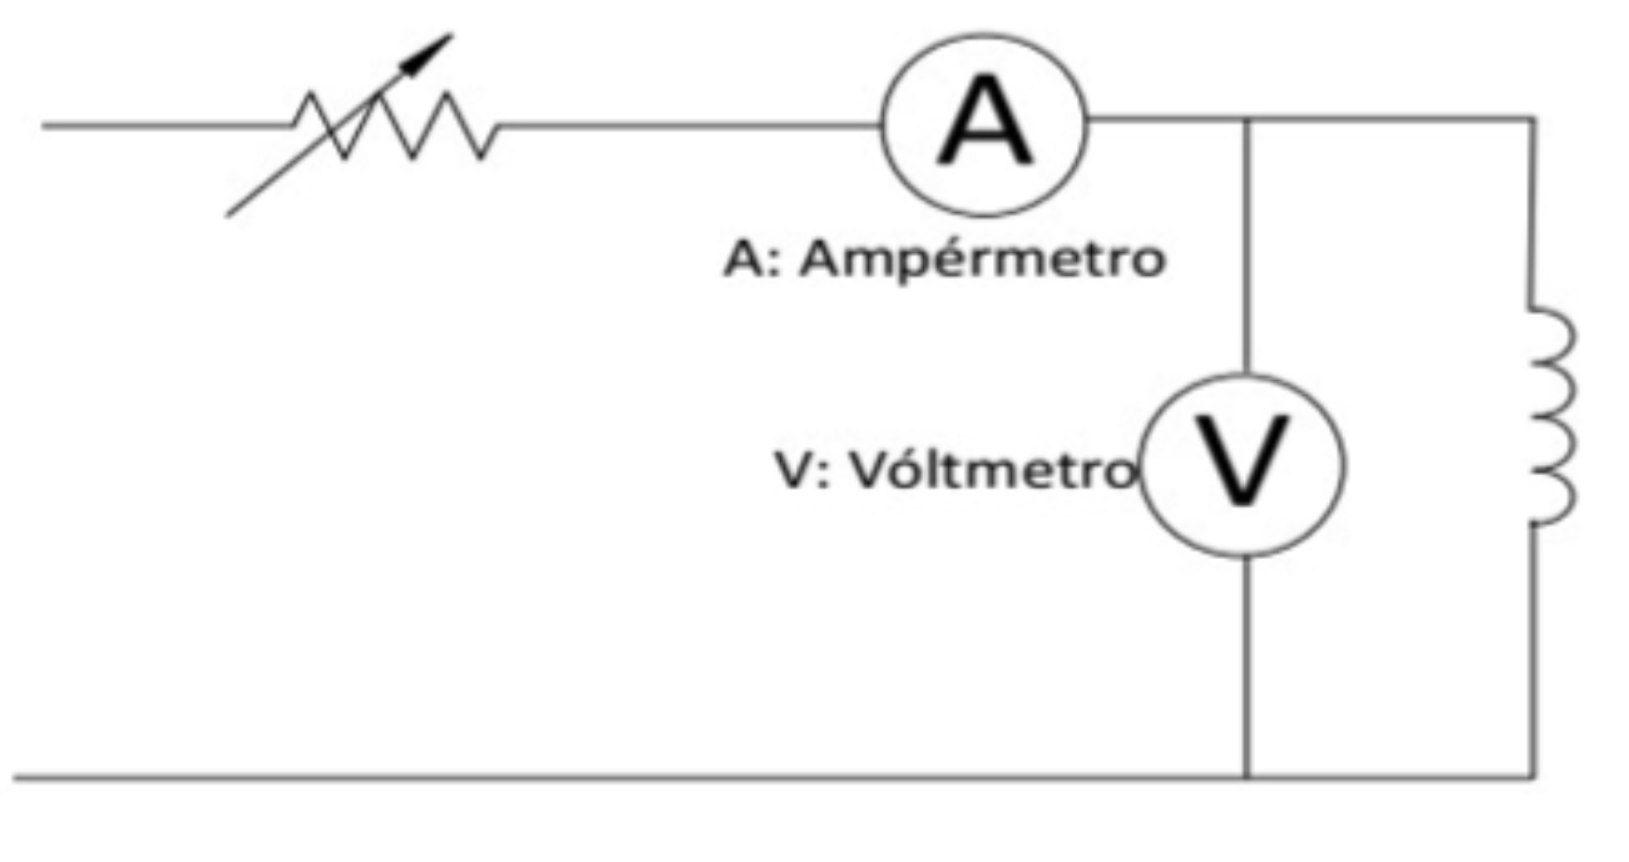
\includegraphics[width=0.48\textwidth]{fot/Prac_6_modelo.png}
    \caption{Topologia de circuito usada para el equivalente.}
    \label{fig:modelol}
\end{figure}


\begin{tabular}{|c|c|c|}
\hline
RESISTENCIA ($\Omega$) & VOLTAJE (V) & CORRIENTE (A) \\
\hline
Máxima & 1.36 & 0.8 \\
2 & 2.020 & 1 \\
3 & 3.560 & 1.49 \\
4 & 5.770 & 2.07 \\
5 (mínima) & 10.93 & 3.60 \\
\hline
\end{tabular}

Con los datos obtenidos anteriormente en la tabla 1, podremos construir la figura \ref{fig:grafica}.
\begin{figure}[ht!]
    \centering
    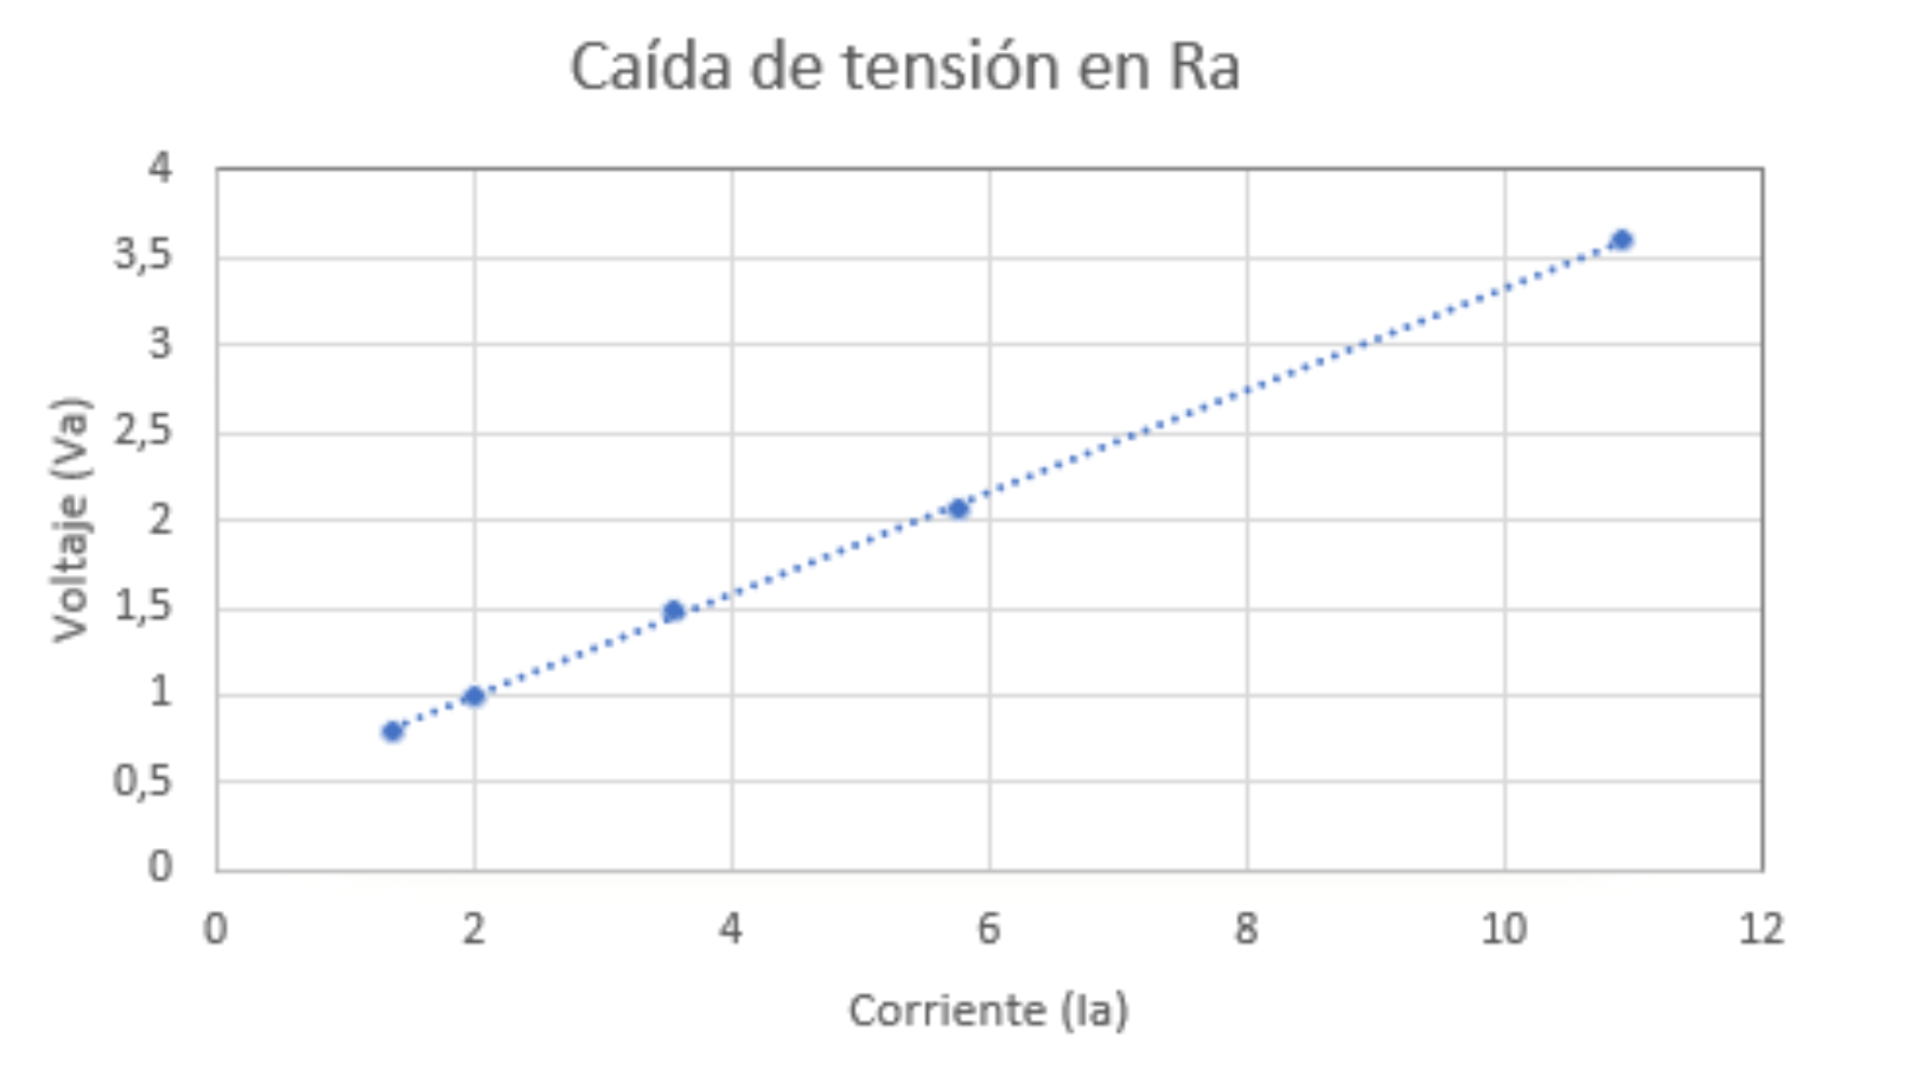
\includegraphics[width=0.48\textwidth]{fot/Prac_6_graf.png}
    \caption{extrapolación de los datos y así obtener la caída de tensión en las escobillas.}
    \label{fig:grafica}
\end{figure}

\textit{Imagen. Gráfica caída de tensión en Ra}

Haciendo la extrapolación con los datos obtenidos y analizándolos de forma lineal, podremos conseguir la caída de tensión en escobillas.

Caída de tensión en escobillas: 0.415518 V

\subsection*{¿Qué es la zona neutra geométrica?}
La zona neutra geométrica en una máquina eléctrica, como un generador o motor de corriente continua (DC), se refiere al área específica del conmutador donde la corriente inducida en los conductores del rotor (inducido) cambia de dirección. Es un concepto crucial para la correcta conmutación y operación de la máquina.
\subsubsection*{Características de la Zona Neutra Geométrica:}
\begin{itemize}
    \item \textbf{Ubicación:} La zona neutra geométrica se encuentra en el plano perpendicular al eje del flujo magnético principal generado por el campo de la máquina. Es decir, está en el lugar donde el flujo magnético es teóricamente cero.
    
    \item \textbf{Función:} En esta zona, las escobillas del motor o generador deben estar posicionadas para que no haya una fuerza electromotriz (fem) inducida en los conductores del inducido cuando están en contacto con las escobillas. Esto reduce las chispas y el desgaste en el conmutador y las escobillas.
    
    \item \textbf{Cambio de dirección de corriente:} A medida que el rotor gira, los conductores pasan por la zona neutra geométrica, cambiando la dirección de la corriente. Este cambio debe ser suave para evitar arcos eléctricos y desgaste prematuro.
\end{itemize}
